\documentclass[a4paper,12pt]{article}

% Packages
\usepackage[utf8]{inputenc}
\usepackage{geometry}
\usepackage{titlesec}
\usepackage{lipsum} % for generating dummy text
\usepackage{graphicx}
\usepackage{caption}
\usepackage{subcaption}
\usepackage{listings}
\usepackage{amsmath}
\usepackage{amssymb}
\usepackage{xcolor}

% Page setup
\geometry{a4paper, margin=1in}
\setlength{\parindent}{0pt}
\setlength{\parskip}{10pt}

% Title setup
\title{\textbf{DSP LAB - LAB 2}}
\author{Ajay Krishnan K \\ EE22BTECH11003}
\date{\today}

% Section and subsection formatting
\titleformat{\section}[block]{\normalfont\Large\bfseries}{\thesection}{1em}{}
\titleformat{\subsection}[block]{\normalfont\large\bfseries}{\thesubsection}{1em}{}
\titleformat{\subsubsection}[block]{\normalfont\normalsize\bfseries}{\thesubsubsection}{1em}{}
% Code listing settings
\lstdefinestyle{mystyle}{
    language=Matlab,
    basicstyle=\ttfamily\small,
    breaklines=true,
    keywordstyle=\color{blue},
    commentstyle=\color{green!40!black},
    stringstyle=\color{red},
    numbers=left,
    numberstyle=\tiny,
    frame=single,
    showspaces=false,
    showstringspaces=false,
}

\lstset{style=mystyle}

\begin{document}
\maketitle

\section{Upsampling}
\subsection{MATLAB}
\subsection*{Code}
\begin{lstlisting}
    % Upsampling using zero insertion

    upsamplingFactor2 = 2;
    upsamplingFactor3 = 3;
    
    x = [0.5377,1.8339,-2.2588,0.8622,0.3188,-1.3077,-0.4336,
        0.3426,3.5784,2.7694,-1.3499,3.0349,0.7254,-0.0631,
        0.7147,-0.2050,-0.1241,1.4897,1.4090,1.4172];
    
    upsampledBy2 = upSample(x, upsamplingFactor2);
    upsampledBy3 = upSample(x, upsamplingFactor3);
    
    disp('Original Signal');
    disp(x);
    disp('Upsampled Signal by 2');
    disp(upsampledBy2);
    disp('Upsampled Signal by 3');
    disp(upsampledBy3);
    
    % Plot the original and upsampled signals
    subplot(3,1,1);
    stem(x, 'b', 'DisplayName', 'Original Signal');
    title('Original Signal');
    xlabel('Sample Index');
    ylabel('Amplitude');
    legend('Original Signal');
    
    subplot(3,1,2);
    stem(upsampledBy2, 'r', 'DisplayName', 'Upsampled Signal by 2');
    title('Upsampled Signal by 2');
    xlabel('Sample Index');
    ylabel('Amplitude');
    legend('Upsampled Signal by 2');
    
    subplot(3,1,3);
    stem(upsampledBy3, 'r', 'DisplayName', 'Upsampled Signal by 3');
    title('Upsampled Signal by 3');
    xlabel('Sample Index');
    ylabel('Amplitude');
    legend('Upsampled Signal by 3');
    
    function y = upSample(x, n)
    N = length(x);
    y = zeros(1, N * n);
    y(1:n:end) = x;
    end
\end{lstlisting}

\subsection*{Output}
\begin{lstlisting}
    Original Signal
      Columns 1 through 17

        0.5377    1.8339   -2.2588    0.8622    0.3188   -1.3077   -0.4336    0.3426    3.5784    2.7694   -1.3499    3.0349    0.7254   -0.0631    0.7147   -0.2050   -0.1241

      Columns 18 through 20

        1.4897    1.4090    1.4172

    Upsampled Signal by 2
      Columns 1 through 17

        0.5377         0    1.8339         0   -2.2588         0    0.8622         0    0.3188         0   -1.3077         0   -0.4336         0    0.3426         0    3.5784

      Columns 18 through 34

             0    2.7694         0   -1.3499         0    3.0349         0    0.7254         0   -0.0631         0    0.7147         0   -0.2050         0   -0.1241         0

      Columns 35 through 40

        1.4897         0    1.4090         0    1.4172         0

    Upsampled Signal by 3
      Columns 1 through 17

        0.5377         0         0    1.8339         0         0   -2.2588         0         0    0.8622         0         0    0.3188         0         0   -1.3077         0

      Columns 18 through 34

             0   -0.4336         0         0    0.3426         0         0    3.5784         0         0    2.7694         0         0   -1.3499         0         0    3.0349

      Columns 35 through 51

             0         0    0.7254         0         0   -0.0631         0         0    0.7147         0         0   -0.2050         0         0   -0.1241         0         0

      Columns 52 through 60

        1.4897         0         0    1.4090         0         0    1.4172         0         0

\end{lstlisting}

\begin{figure}[h!]
    \centering
    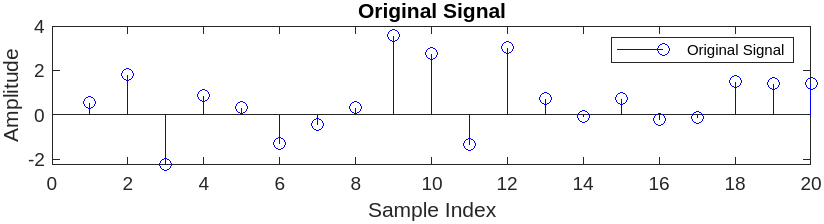
\includegraphics[width=0.8\textwidth]{figs/og_up.png}
    \caption{Upsampling Sample Signal}
    \label{fig:upsampling}
\end{figure}

\begin{figure}[h!]
    \centering
    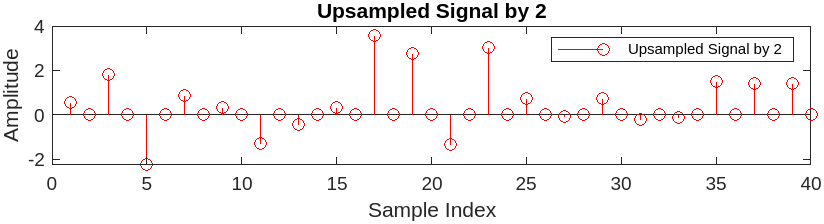
\includegraphics[width=0.8\textwidth]{figs/2_up.png}
    \caption{Upsampling by Factor of 2}
    \label{fig:upsampling_2}
\end{figure}

\begin{figure}[h!]
    \centering
    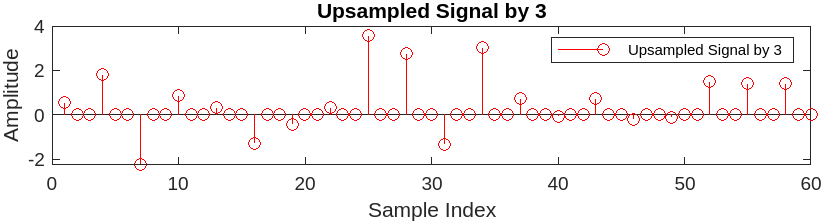
\includegraphics[width=0.8\textwidth]{figs/3_up.png}
    \caption{Upsampling by Factor of 3}
    \label{fig:upsampling_3}
\end{figure}

\newpage
\subsection{C}

\subsection*{Code}

\begin{lstlisting}
    #include <stdio.h>

    void upsampleSignal(float input[], int inputSize, float output[], int n)
    {
        int outputSize = inputSize * n;
        int index = 0;

        for (int i = 0; i < inputSize; i++)
        {
            output[index++] = input[i];
            for (int j = 1; j < n; j++)
            {
                output[index++] = 0.0;
            }
        }
    }

    int main()
    {
        int inputSize = 20;
        float input[20] = {0.5377, 1.8339, -2.2588, 0.8622, 0.3188, -1.3077, -0.4336, 0.3426, 3.5784, 2.7694, -1.3499, 3.0349, 0.7254, -0.0631, 0.7147, -0.2050, -0.1241, 1.4897, 1.4090, 1.4172};
        int upsampleSignal2 = 2;
        int upsampleSignal3 = 3;
        int outputSize2 = inputSize * upsampleSignal2;
        int outputSize3 = inputSize * upsampleSignal3;
        float output2[outputSize2];
        float output3[outputSize3];

        upsampleSignal(input, inputSize, output2, upsampleSignal2);
        upsampleSignal(input, inputSize, output3, upsampleSignal3);

        printf("Input Signal: ");
        for (int i = 0; i < inputSize; i++)
        {
            printf("%f ", input[i]);
        }

        printf("\nUpsampled Signal by 2: ");
        for (int i = 0; i < outputSize2; i++)
        {
            printf("%f ", output2[i]);
        }

        printf("\nUpsampled Signal by 3: ");
        for (int i = 0; i < outputSize3; i++)
        {
            printf("%f ", output3[i]);
        }

        return 0;
    }

\end{lstlisting}

\subsection*{Output}
\begin{lstlisting}
    Input Signal: 0.537700 1.833900 -2.258800 0.862200 0.318800 -1.307700 -0.433600 0.342600 3.578400 2.769400 -1.349900 3.034900 0.725400 -0.063100 0.714700 -0.205000 -0.124100 1.489700 1.409000 1.417200 
    Upsampled Signal by 2: 0.537700 0.000000 1.833900 0.000000 -2.258800 0.000000 0.862200 0.000000 0.318800 0.000000 -1.307700 0.000000 -0.433600 0.000000 0.342600 0.000000 3.578400 0.000000 2.769400 0.000000 -1.349900 0.000000 3.034900 0.000000 0.725400 0.000000 -0.063100 0.000000 0.714700 0.000000 -0.205000 0.000000 -0.124100 0.000000 1.489700 0.000000 1.409000 0.000000 1.417200 0.000000 
    Upsampled Signal by 3: 0.537700 0.000000 0.000000 1.833900 0.000000 0.000000 -2.258800 0.000000 0.000000 0.862200 0.000000 0.000000 0.318800 0.000000 0.000000 -1.307700 0.000000 0.000000 -0.433600 0.000000 0.000000 0.342600 0.000000 0.000000 3.578400 0.000000 0.000000 2.769400 0.000000 0.000000 -1.349900 0.000000 0.000000 3.034900 0.000000 0.000000 0.725400 0.000000 0.000000 -0.063100 0.000000 0.000000 0.714700 0.000000 0.000000 -0.205000 0.000000 0.000000 -0.124100 0.000000 0.000000 1.489700 0.000000 0.000000 1.409000 0.000000 0.000000 1.417200 0.000000 0.000000
\end{lstlisting}

\section{Downsampling}
\subsection{MATLAB}
\subsection*{Code}
\begin{lstlisting}
    % Downsampling

    downsamplingFactor2 = 2;
    downsamplingFactor3 = 3;
    
    x = [0.5377,1.8339,-2.2588,0.8622,0.3188,-1.3077,-0.4336,
        0.3426,3.5784,2.7694,-1.3499,3.0349,0.7254,-0.0631,
        0.7147,-0.2050,-0.1241,1.4897,1.4090,1.4172];
    
    downsampled_2 = downSample(x, downsamplingFactor2);
    downsampled_3 = downSample(x, downsamplingFactor3);
    
    % Plot the original and downsampled signals
    subplot(3,1,1);
    stem(x, 'b', 'DisplayName', 'Original Signal');
    title('Original Signal');
    xlabel('Sample Index');
    ylabel('Amplitude');
    legend('Original Signal');
    
    subplot(3,1,2);
    stem(downsampled_2, 'r', 'DisplayName', 'Downsampled by 2');
    title('Downsampled Signal');
    xlabel('Sample Index');
    ylabel('Amplitude');
    legend('Downsampled by 2 Signal');
    
    subplot(3,1,3);
    stem(downsampled_3, 'r', 'DisplayName', 'Downsampled by 3');
    title('Downsampled Signal');
    xlabel('Sample Index');
    ylabel('Amplitude');
    legend('Downsampled by 3 Signal');
    
    function y = downSample(x, n)
    y = x(1:n:end);
    end
    
\end{lstlisting}

\subsection*{Output}
\begin{lstlisting}
    Original Signal
      Columns 1 through 17

        0.5377    1.8339   -2.2588    0.8622    0.3188   -1.3077   -0.4336    0.3426    3.5784    2.7694   -1.3499    3.0349    0.7254   -0.0631    0.7147   -0.2050   -0.1241

      Columns 18 through 20

        1.4897    1.4090    1.4172

    Downsampled by 2 Signal
        0.5377   -2.2588    0.3188   -0.4336    3.5784   -1.3499    0.7254    0.7147   -0.1241    1.4090

    Downsampled by 3 Signal
        0.5377    0.8622   -0.4336    2.7694    0.7254   -0.2050    1.4090
\end{lstlisting}

\begin{figure}[h!]
    \centering
    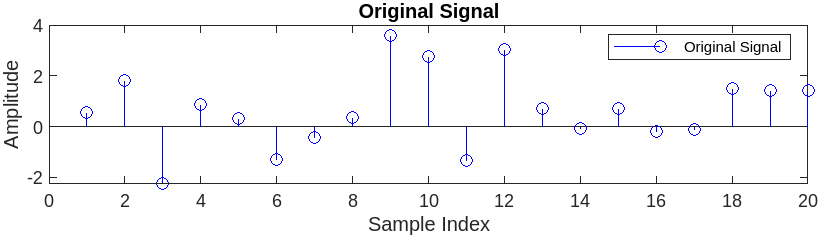
\includegraphics[width=0.8\textwidth]{figs/og_down.png}
    \caption{Downsampling Sample Signal}
    \label{fig:downsampling_original}
\end{figure}

\begin{figure}[h!]
    \centering
    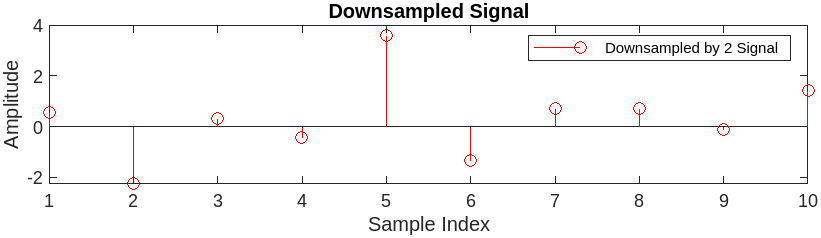
\includegraphics[width=0.8\textwidth]{figs/2_down.png}
    \caption{Downsampling Signal by Factor of 2}
    \label{fig:downsampling_2}
\end{figure}

\begin{figure}[h!]
    \centering
    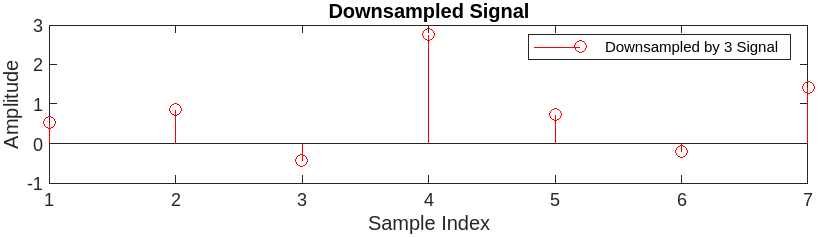
\includegraphics[width=0.8\textwidth]{figs/3_down.png}
    \caption{Downsampling Signal by Factor of 3}
    \label{fig:downsampling_3}
\end{figure}


\newpage

\subsection{C}

\subsection*{Code}
\begin{lstlisting}
    #include <stdio.h>

    void downsampleSignal(float input[], int inputSize, float output[], int n)
    {
        int outputSize = inputSize / n;
        int index = 0;
    
        for (int i = 0; i < inputSize; i += n)
        {
            output[index++] = input[i];
        }
    }
    
    int main()
    {
        int inputSize = 20;
        float input[20] = {0.5377, 1.8339, -2.2588, 0.8622, 0.3188, -1.3077, -0.4336, 0.3426, 3.5784, 2.7694, -1.3499, 3.0349, 0.7254, -0.0631, 0.7147, -0.2050, -0.1241, 1.4897, 1.4090, 1.4172};
        int downsampleFactor2 = 2;
        int downsampleFactor3 = 3;
        int outputSize2 = inputSize / downsampleFactor2;
        int outputSize3 = inputSize / downsampleFactor3;
        float output2[outputSize2];
        float output3[outputSize3];
    
        downsampleSignal(input, inputSize, output2, downsampleFactor2);
        downsampleSignal(input, inputSize, output3, downsampleFactor3);
    
        printf("Input Signal: ");
        for (int i = 0; i < inputSize; i++)
        {
            printf("%f ", input[i]);
        }
    
        printf("\nDownsampled Signal by 2: ");
        for (int i = 0; i < outputSize2; i++)
        {
            printf("%f ", output2[i]);
        }
    
        printf("\nDownsampled Signal by 3: ");
        for (int i = 0; i < outputSize3; i++)
        {
            printf("%f ", output3[i]);
        }
    
        return 0;
    }

\end{lstlisting}

\subsection*{Output}

\begin{lstlisting}
    Input Signal: 0.537700 1.833900 -2.258800 0.862200 0.318800 -1.307700 -0.433600 0.342600 3.578400 2.769400 -1.349900 3.034900 0.725400 -0.063100 0.714700 -0.205000 -0.124100 1.489700 1.409000 1.417200 
    Downsampled Signal by 2: 0.537700 -2.258800 0.318800 -0.433600 3.578400 -1.349900 0.725400 0.714700 -0.124100 1.409000 
    Downsampled Signal by 3: 0.537700 0.862200 -0.433600 2.769400 0.725400 -0.205000
\end{lstlisting}

\end{document}